% Chapter Template

\chapter{Method} % Main chapter title

\label{Chapter3} % Change X to a consecutive number; for referencing this chapter elsewhere, use \ref{ChapterX}

%----------------------------------------------------------------------------------------
%	SECTION 1
%----------------------------------------------------------------------------------------

\section{Evolutionary Algorithm: HyperNEAT} \label{sec:method_hyperneat}

HyperNEAT \cite{StanleyDAmbrosioGauci2009} is an extension of NEAT (\textit{Neuro-Evolution of Augmented Topologies})
\cite{StanleyMiikkulainen2002}, where ANNs are indirectly encoded using a CPPN (\textit{Compositional Pattern Producing Network})
\cite{Stanley2007}.
HyperNEAT was selected as it has a number of benefits demonstrated in previous work \cite{DAmbrosio2013},
\cite{WatsonNitschke2015SSCI}.
This includes its capability to exploit geometric features such as symmetry, regularity and modularity
in robot morphology and the task environment during controller evolution.
%in the  geometric features include the relative positions of other robots, blocks,
%the direction robots and blocks are facing and the shape of the environment.
%Also, the structures to be built are modular
%(comprised of blocks) and often regular (the same sequence of blocks can be repeated).

The nodes comprising each robot's ANN controller, connected by the CPPN, were placed in the substrate
illustrated in figure \ref{fig:ann}.

Each node in the substrate was placed at specific ($x$, $y$) locations in the two-dimensional geometric space
of the substrate ($x$, $y$ axes were in the range: [-1, 1]).

Connection weights in the controller were evolved via querying the CPPN for the weight of any connection
between two points ($x_{1}$, $y_{1}$) and ($x_{2}$, $y_{2}$) by inputting ($x_{1}$, $y_{1}$, $x_{2}$, $y_{2}$)
into the CPPN, which subsequently output the associated weight.

During HyperNEAT's evolutionary process, the CPPN was evolved via having nodes and connections added and removed, as well
as connection weight values mutated \cite{StanleyDAmbrosioGauci2009}.

Thus, the CPPN evolved a connectivity pattern across the geometry of the ANN via querying all the potential
connections for their weights.

This connectivity pattern was effectively a function of the task and ANN geometry,
which enabled HyperNEAT to exploit the structure (regularity, repetition and symmetry) of the task and robot morphology.

For example, there was symmetry in the robot morphology in terms of the positioning of sensors about each
robot's periphery (figure \ref{fig:ann}) and there was regularity and repetition in the collective construction
task, in terms of repeating block types comprising modular and regular structures.

In the collective construction task, \textit{modularity} was defined as the composition of modular structures
(buildings in construction zones) from a sequence of connected blocks and \textit{regularity} was defined
as the same sequence of blocks repeated in a building.

Previous work has demonstrated that the indirect encoding of an evolved CPPN facilitates the evolution of
robot controllers with increased task performance enabled by a compact representation
of task and robot geometry \cite{DAmbrosioStanley2008}, \cite{WatsonNitschke2015SSCI}.

Table \ref{tab:simParameters} presents the HyperNEAT parameters used in this study, where \textit{delta}
was angle between the ($x_{1}$, $y_{1}$, $x_{2}$, $y_{2}$) positions of nodes in the substrate.
These parameter values were determined experimentally.   All other HyperNEAT parameters not listed in
table \ref{tab:simParameters}, were set as in previous work \cite{DAmbrosioStanley2008}.


			%%%%%%%%%%%%%%%%%%%%%%%%%%%%%%%%%%%%%%%%%%%%%%%%%%%%%%%%%%%%%%
			%% 				From the AAMAS Extended Abstract			%% 
			%%					Methods and Experiments					%%
			%%%%%%%%%%%%%%%%%%%%%%%%%%%%%%%%%%%%%%%%%%%%%%%%%%%%%%%%%%%%%%

HyperNEAT was applied to evolve robot team (collective) behaviours, where teams were behaviourally and morphologically homogeneous teams meaning all robots in a given team used the same controller and sensory configuration.

\section{ANN Controller}

Each robot in the team used an ANN controller with
\textit{N} sensory input nodes, determined by the given morphology being evaluated (table \ref{tab:morphConfigs}).
Each robot's controller mapped sensory inputs, via a fully connected hidden layer, to two motor outputs, the
robot's left and right wheels (figure \ref{fig:ann}). %using HyperNEAT \cite{StanleyDAmbrosioGauci2009}.

Figure \ref{fig:ann} illustrates the sensory configuration for \textit{N} = $11$ (morphology $1$), and the
associated substrate and CPPN used by HyperNEAT.

For each robot morphology (table \ref{tab:morphConfigs}), the sensors corresponding to the input layer
of the controller was a circle \textit{N} nodes distributed about a robot's periphery,
where the exact geometric configuration corresponded to the morphology being evaluated
(figure \ref{fig:ann} illustrates morphology
$1$)\footnote{Illustrations of all robot morphologies tested can be found at: \url{https://github.com/not-my-name/SSCI_Paper_Appendix}}.

The intermediate ANN hidden layer reflects the configuration of the input layer, preserving
the geometry of the sensory input layer, that is, the direction of each sensor's FOV (figure
\ref{fig:ann}).

The ANN was initialized with random weights normalized to the range [-1.0, 1.0], with full connectivity between adjacent layers.

That being said, it was still possible to evolve partial connectivity via the CPPN generating a zero weight for a connection between 2 nodes from adjacent layers.

Collectively all sensors approximated up to a $360$ degree \textit{Field of View} (FOV).


%The ANN uses a three dimensional coordinate system for processing \textit{x}, \textit{y}, \textit{z}
%positions in the CPPN in order to generate weight and bias values and connectivity.
%Previous work  also demonstrated that HyperNEAT exploits the sensory-motor node configuration in ANN controllers,
%Nodes for processing sensory inputs correspond to the direction each sensor faces.

\begin{table*} [t]
	\renewcommand{\arraystretch}{1.50}
	\caption{Sensory configuration (number of sensors) for each morphology.}\label{tab:morphConfigs}
	\centering
	\begin{tabular}{| c | c | c | c | c | c |}
		\hline
\textbf{Morphology ID} & \textbf{Proximity Sensors} & \textbf{Ultrasonic Sensors} & \textbf{Color Ranged Sensors} & \textbf{Low-Resolution Camera} & 	 \textbf{Construction Zone Sensors} \\
%                       &   Sensors     &   Sensors          &  Sensors         &   Camera          &   Zone Sensors \\
		\hline
		\textbf{1}               &	5 	 	    & 	3  	             &	1               &	1                &	1   \\
		\textbf{2}               &	4 	 	    &	1		         &	1	            &	1                &	1   \\
		\textbf{3}               &	0 	        &	0				 &	1			    &	1                &	1    \\
		\textbf{4}               &	2 		 	&	0	     		 &	1		        &	1                &	1    \\
		\textbf{5}               &	2  	        & 	2				 &  1               &	1                &	1    \\
		\hline
	\end{tabular}
\end{table*}

\subsection{Input Sensors}

Each robot was equipped with various sensor types, where the exact sensor complement, including the
relative position and direction on the robot depends upon the given experiment
(section \ref{sec:experiments}) and morphology being evaluated (table \ref{tab:morphConfigs}).

Each robot had \textit{N} sensors corresponding to the \textit{N} inputs comprising the robot's
ANN sensory input layer (figure \ref{fig:ann}), each with a range of \textit{r}
(portion of the environment's length).

A robot's sensory FOV was split into \textit{N} sensor quadrants, where all sensors were constantly active
for the duration of the robot's lifetime (unless stated otherwise in experiment conditions).

The \textit{nth} sensor returned a value in the normalized range [0.0, 1.0],
in the corresponding \textit{nth} sensor quadrant.

A value of $0.0$ indicated that no blocks were detected and a value of $1.0$ indicated that an object was detected
at the closest possible distance to the given sensor.
%All detection sensor values are

Table \ref{tab:simParameters} presents the different sensor types used in this study, where the functional properties of each sensor
(range and FOV) were abstractions of corresponding physical sensors typically used on the Khepera III robots \cite{khepera3usermanual2013}.

In table \ref{tab:simParameters}, range values are units defined in relation to the environment size ($20$ x $20$)
and FOV values are in radians.

Each morphology also included a special construction zone detection sensor that activated with a value in the range
[0.0, 1.0] whenever a robot came into
contact with a block that must be connected with other already connected blocks (existing construction zones).

The construction zone sensor calculated the squared Euclidean norm, bounded by a minimum observation distance, as an
inversely proportional distance between \textit{this} robot and the closest construction zone, where a value of 1.0 indicated the robot (pushing a block)
was in contact with the construction zone and a value of 0.0 indicated that the robot (pushing a block) was the maximum possible
distance from the closest construction zone.

Robots were unable to detect each other, thus all cooperative interactions were \textit{stigmergic} \cite{BeckersHollandDeneubourg1994}
where robots interacted via pushing blocks into the environment's construction zone.

Furthermore, robots had no \textit{a priori} knowledge of the construction schema,
but rather must discover the construction schema rules by trial and error.

Also, once at least two blocks had been pushed and connected together this formed a construction zone (section \ref{subsec:constructionTask}),
that was then visible to each robot's construction zone sensor.
%Each robot has \textit{N} sensors each with a specified range, field of view and bearing (its position on the robot). The subject of these experimental comparisons is the various combinations of these different types of sensors (referred to as sensor morphologies) that are implemented in the different experiments. These sensor morphologies are predetermined by the experimenter and are outlined later on in this table. Robots are unable to detect each other, thus all cooperative interactions are \textit{stigmergic} \cite{BeckersHollandDeneubourg1994}

\subsection{Movement Actuators}

These movement actuators correspond to the output nodes for each ANN controller.

Two wheel motors control a robot's heading at constant speed.
Movement is calculated in terms of real valued vectors (\textit{dx}
and \textit{dy}).  Wheel motors (\textit{L} and \textit{R} in figure \ref{fig:ann})
need to be explicitly activated.
A robot's heading is determined by normalizing and scaling its motor
output values by the maximum distance a robot can traverse in one
iteration (table \ref{tab:simParameters}).  That is:

%\begin{equation}\label{equ:contDisCalc}
$\textit{dx} = d_{max} (o_{1} - 0.5)$

$\textit{dy} = d_{max} (o_{2} - 0.5)$
%\end{equation}

Where, $o_{1}$ and $o_{2}$ are the motor output values, corresponding
to the left and right wheels, respectively, producing an output in the range:
[-1.0, 1.0].
These output values indicate how fast each respective wheel must turn.
Equal output equates to straight forward motion and unequal output results
in the robot rotating about its own axis.
The $d_{max}$ value indicates the maximum distance a robot can move in
one simulation iteration (normalized to 1.0, table \ref{tab:simParameters}).



\begin{figure}[t]
	\centering
	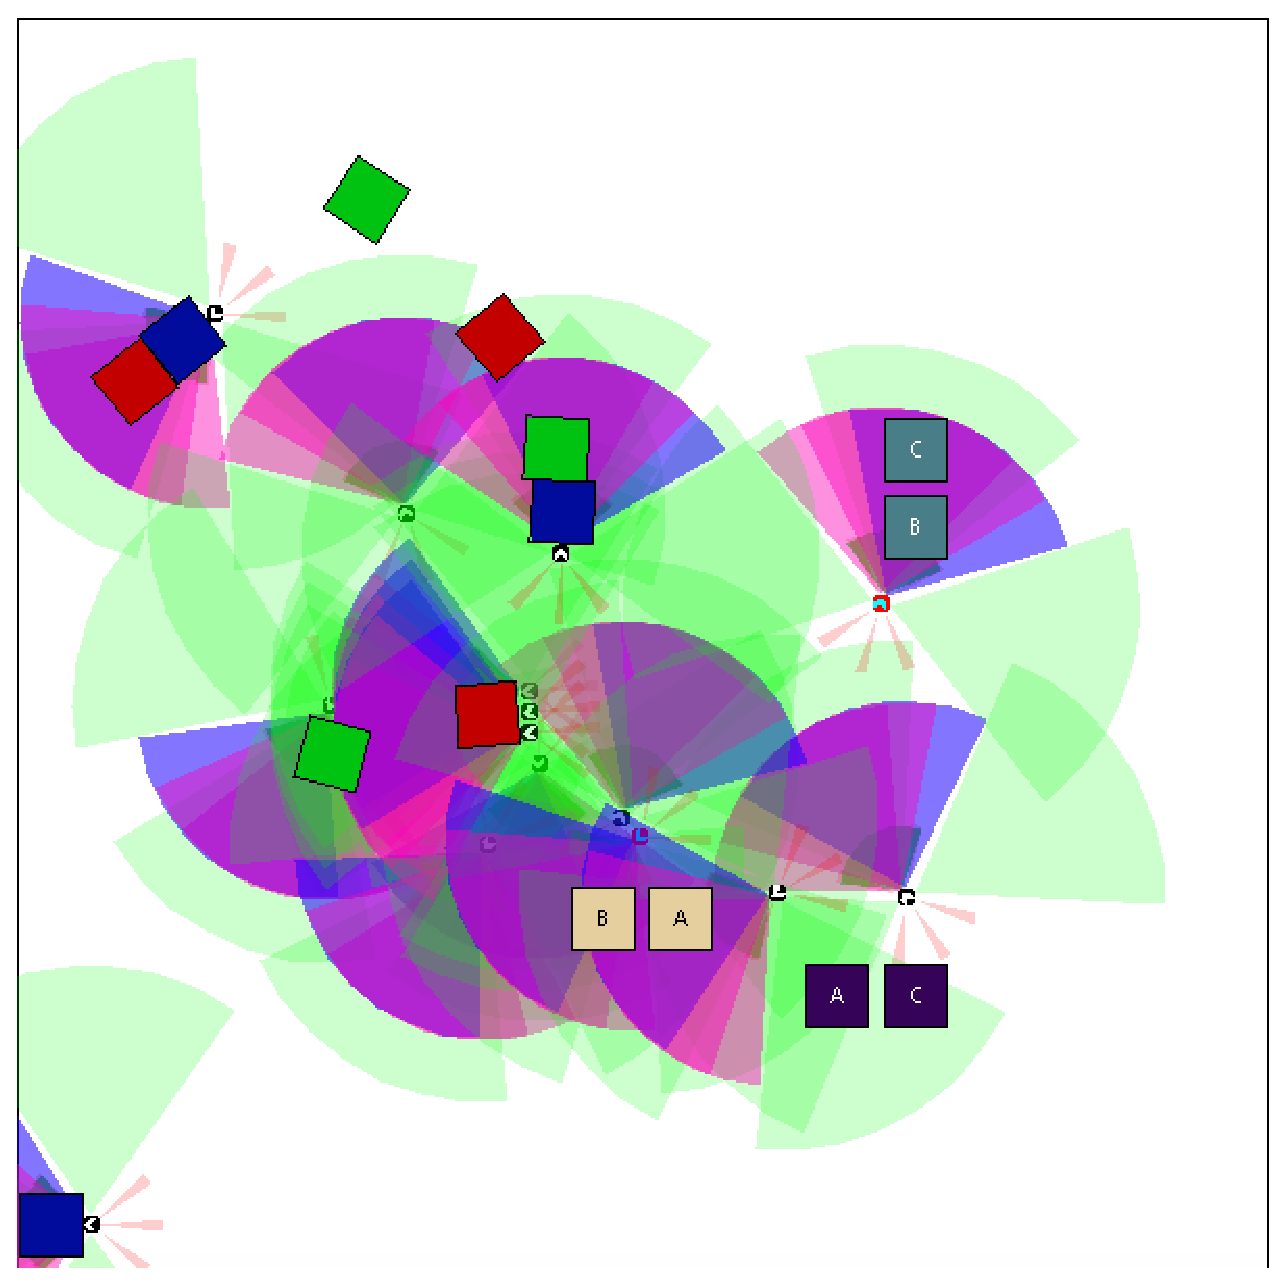
\includegraphics[width=0.40\textwidth]{TaskEnv.eps}
\caption{Example of the simulation environment.  Robots search for randomly distributed
type A, B, and C blocks (blue, green and red, respectively).  Other colored and labeled
blocks indicate those already connected in construction zones.
Different coloured semi-circles emanating from each
robot represent the field of view of currently active different sensor types (table \ref{tab:simParameters}).}\label{fig:taskEnv}
\end{figure}




\section{Simulated Environment}

These experiments were conducted in a simulated 2-dimensional environment that made use of the Redbridge simulator {insert a reference}

The robots that were used were simplified and abstracted versions of the Khepera robots (maybe find an online reference to what they are). This because they are relatively simple and cheap to buy and they are also compatible with a wide range of sensors.

The physics of the simulated environment were relatively basic. It was implemented by using the JBox2D library for Java.

The environment through which the agents move and in which they interact is continous space but the environment results are evaluated using an underlying discretised grid. This is also used to 'snap' the connected resources to a fixed location on the grid once it has been attached to the construction zone. This is determined by checking the resource's distance to a connection surface as well as the its orientation relative to the target bloc. If it is within an acceptable range, the block automatically snaps into place and becomes fixed in space.

This toolkit is written in Java and it was chosen because of its consistent performance across a range of machines and its compatibility with various operating systems which would be useful in the testing phase as we had to run the simulations on a number of machines.

One of the reasons for choosing the MASON Java library is because it can easily be integrated with other Java-based tools, such as the Encog Machine Learning library, which is discussed earlier on in this section (\ref{sec:method_hyperneat}).

\subsection{Construction Zone}

A construction zone refers to an already existing structure that consists of two or more connected resources.
Some examples of construction zones are shown in the following diagram (insert an illustration) and are indicated by the connected blocks changing to the same colour as well as having a label indicating the blocks type.

This is a collection of already constructed resources. It can be thought of as the current object that is currently under construction. This is the structure to which new resources should be connected in order to accomplish the construction of a single cohesive object rather than just a bunch of small structures that consist of 2 or 3 blocks.

Once a resource has been connected to a construction zone it becomes fixed in place. The entire construction zone is static and once a resource has been connected to it, it can not be disconnected again.

In order to encourage the construction of a single structure rather than just scattered structures that consist of 2 or 3 connected blocks, we restricted the number of construction zones to 3 per simulation. This means that 2 'free' resources can only be connected to each other thrice, the rest of the (subsequent) resources must be connected to one of those existing construction zones 
'This only gets done for the first three pairs of blocks in order to encourage the development of a singular structure instead of several smaller ones'

The fact that the construction zones are only created by whichever 2 resources are connected first means that the location of the construction zone is different for each simulation run and depends on where the robots connect the first 2 blocks.

\subsection{Resource Blocks}

In order to represent the raw materials that are scattered throughout the environment for which the agents must search, we made use of basic squares with different physical properties.

These properties include:
-> How many robots need to cooperate in order to be able to move the construction block
-> Which types of blocks can be connected on which specific sides of the construction block (these are referred to as the underlying construction schema).

Three different types of construction blocks were implemented in order to define the complexity/difficulty of the task at hand

The complexity of the task is defined by the simulated environment and the resources that are present within it.

\subsection{Construction Rules / Task Complexity}

The level of required cooperation and the complexity of each experiment is determined by the types of blocks present in the environment (cooperation to move heavier blocks) and whether or not there are any construction rules present in the current schema.

An illustrated example of how the various difficulty levels are implemented is shown in figure \ref{fig:constructionSchema}.
Additionally, these configurations are outlined in more details later on in table \ref{tab:taskComplexity}.

(Used to implicitly define the complexity of the simulated task at hand by controlling the simulated environment)

The connection schema specifies the number of each type of construction block that is to be placed in the environment for a specific experiment level. 

\begin{figure}[t]
	\centering
	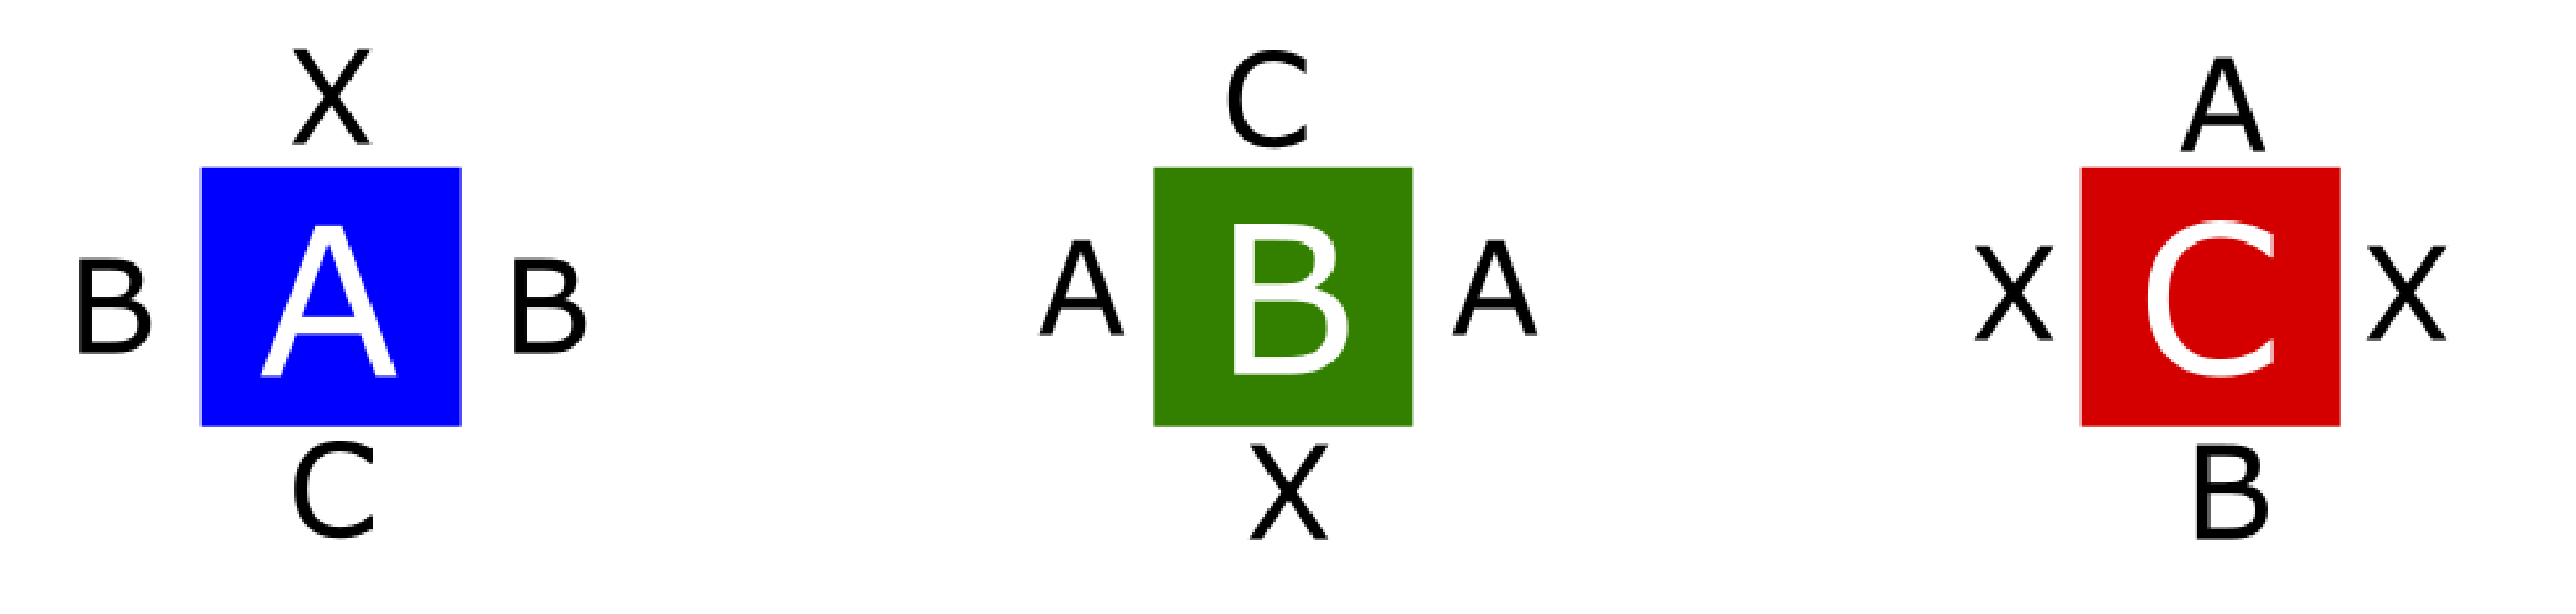
\includegraphics[width=0.5\textwidth]{ConstructionSchema.PNG}
	\caption{Task level 3 construction schema: \textit{A}, \textit{B}, and \textit{C} are the block types.  The label on
each side of each block type indicates what block type can be connected to this side.  An \textit{X} label indicates
that no block can be connected.}\label{fig:constructionSchema}
\end{figure}

Figure \ref{fig:constructionSchema} provides an illustrated version of the various types and numbers of resource blocks that are present for each experiment level.

Level $1$ was the least complex as it did not require
any cooperation, given that in this case there were only type \textit{A}
blocks in the environment.

Level $2$ was of medium complexity as there are equal numbers of type \textit{A},
\textit{B}, and \textit{C} blocks in the environment, where block types \textit{B} and \textit{C} required
at least two and three robots to push, respectively.

Level $3$ was the most complex, as it required the same degree of cooperation as task level
$2$, though blocks had to be connected according to a construction schema.
Figure \ref{fig:constructionSchema}
illustrates this construction schema, where the label on each of the
four sides of each block type indicates what other block type can be connected to the given side.

When block types have no letters on the sides it means that there were no blocks of that type present in the environment for that complexity level of the simulation (as with block types B and C in the first level of the illustrated schema)

\section{Collective Construction Task}

\hl{should this section not perhaps be part of the introduction section}

The collective construction task was chosen as it is a task that benefits from autonomous robot groups that must exhibit robust collective behaviour in dynamic, noisy environments. Also, the collective construction task includes the notion of morphological damage to robots that may impede group task accomplishment. 

The collective construction task requires that a team of agents cooperate by coordinating their behaviours in order to assemble various structures within their environment [reference] <verbatim from the honours paper>
In this case, a team of homogeneous robots needs to search for various types of construction block scattered throughout the environment and connect them in order to construct a single large structure. 

The collective construction task can be sub-divided into three smaller sub-tasks:
	First:
		the robots need to search the environment in order to find the loose construction blocks.
	Second:
		once a robot has located a block, it needs to pick it up and move it towards a construction zone. If there is no previously existing/created construction zone, then it needs to move the block towards another block in order to start a new construction zone. A new construction zone is created when any 2 free resources are successfully connected.
	Third:
		the robot must then try to connect the block it's carrying either to an existing construction zone or another block (to start a new construction zone). Once the robot has succcessfully connected the block to a construction zone, it releases the block and starts the process again by searching for another free block.

The robots need to cooperate in order to collect and construct the heavier block types.

The controller also needs to learn the underlying connection rules specified by the schema in order to be able to connect the appropriate block types to each other.




\subsection{Task Complexity}

The complexity of the collective construction task is controlled by implementing the different connection schemas. By requiring the robots to cooperate in order to be able to move certain block types and implementing connection rules, it is necessary to evolve more complex controllers that are able to account for cooperative interactions which is a non-trivial task for most Evolutionary Algorithms (should maybe find a reference for this past paragraph? Currently its taken straight from page 5 of honours paper)

The controllers that were produced using HyperNEAT and the various fitness functions were evaluated based on how successful they were at solving the collective construction task. A controller's task performance is defined by the number of different types of blocks that it managed to connect to a construction zone.

Each of the different types of construction blocks are worth a different score depending on what level of cooperation they require (how many agents it takes to move the block)
"I dont think there is any reward calculation for the complexity of the construction schema" The point is to simply deploy the agents with a more complex schema and then just see if they are able to solve the same task. I dont think its necessary to account for the difficulty level of the simulation in the fitness function calculation.

\subsection{Construction Schema}

The complexity/difficulty of a given simulation level is determined by the types of construction blocks present in the environment (as this determines the level of cooperation) as well as then underlying connection rules that govern which blocks can be connected to which other blocks and on their corresponding sides.

These underlying connection rules are specified using what will be referred to as a construction schema. This is essentially just a YAML file that indicates what block types can be attached to which side of each respective block. Whenever the robots attempt to connect 2 construction blocks, the simulator refers to this file and checks that the construction schema allows for these blocks to be connected on the indicated sides.

This is almost like an abstract representation of how receptors and hormones work in the brain, i think. Or is it something to do with DNA replication? Eitrher way, its like the lock-key model for proteins

This is analogous to the way in which puzzle pieces only fit together on specific sides and orientations.

When a robot attempts to attach 2 blocks to each other, the connection rules for both blocks must be satisfied in order for a successful connection to be made.


\section{Team Controller}

'This is from the GECCO Penultimate paper pg2, remember to go get the references and the diagrams'

Each robot's ANN controller comprised N sensory input and hidden nodes, connected hidden layer to two motor outputs (controlling the robot's left and right wheels). Nodes were arranged as a substrate where the number of input and hidden nodes was determined by a give robot morphology. Each substrate node was placed at specific (x,y) locations in the substrate's two-dimensional geometric space. Sensor nodes of the substrate approximated up to a 360deg sensory FOV, where the FOV was dependent on the morphology used.































